\chapter{Mission: Datacenter}

\emph{\emph{Datacenter} is a doubles team mission on a~4'x4' play area
  and with~300 army points per side in which the alliances attempt to
  secure Dr Tokh's most valuable data from a major campus computing
  cluster.}

\section{Play Area}
\vspace{-2\parskip}
\noindent\begin{stdminipage}{\linewidth-(4in+1.5em)}
\vspace{0pt}   

The Deployment Zones are~12'' areas along opposing play area edges.

Nine Server objectives are placed in a grid: Three on the centerline
between the deployment zones, one at the center and the other two~12''
from each edge; and six in two lines of three~8'' from that centerline
in each half of the play area, each with one at the center and the
other two~12'' from each edge.

Each Server is randomly assigned a Data Topic without it being
revealed to either team, via markers placed facedown next to them.
There are three each of three Data Topics: Bio/Xeno, Cyber, and MechE.

\section{Mission Rules}

%   Teams whose alliance controls more
% Quadrants than their opponents' receive a~+3 MOD to this roll.

%  \href{http://wiki.infinitythegame.com/en/index.php?title=Initiative_and_Deployment}{}

The Connect Objective short skill may be applied to Servers in this
mission.

\end{stdminipage}
\hfill
\begin{minipage}[t]{4in}\centering
\vspace{4pt}   
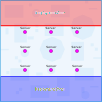
\includegraphics{maps/map-datacenter}
\end{minipage}

Teams may look at the assigned Data Topic for any Server they have
connected at any time.  In addition, Network Directory tokens earned
by teams in the preceding missions may be discarded to look at the
assigned Data Topic for up to three Servers per token.  In neither
case are the Data Topics revealed to the other team.  Teams may keep
secret notes about what they have learned of the Servers.

\section{Scoring}

Teams may score up to~20 objective points via the following conditions
at game end:
\begin{squishitemize}
\item 1pt for each Data Topic of which the team is connected to at
  least one Server.
\item 2pts for each Data Topic of which the team is connected to the
  most Servers.
\item 1pt for being connected to at least one Server for each of the
  three Data Topics.

\item 2pts for each friendly Special Agent in base contact with a
  Server (connected or otherwise).
\item 2pts for each friendly Special Agent wholly in the enemy half of
  the play area.
\item 1pt for each opposing Special Agent in a Null State or
  eliminated.

% \item 1pt if at least~50\% of your army list by points has survived.
%\item 1pt if more points of the opposing army list have been destroyed.
\end{squishitemize}
